\subsection{Optimization problem}

In section \ref{MDP}, it's described that the problem of
find a policy that allows an agent to play Tetris well
cannot be approached with pure analytical methods.
When applying the more% viable \textit{Monte Carlo} methods
to assess the value function of a policy, the only 
knowledge one gains is the actual value from the estimation 
of the value function. Algorithms such as the Cross Entropy Method
and CMA are both designed to solve exactly these types of problems.
The rest of this section is devoted to present the properties of the 
general problem to be solved by the two algorithms, and how the 
problem of optimizing Tetris fits within this model.

\subsubsection{General problem}

The general problem that the Cross Entropy Method and CMA 
tries to solve is often referred  to as a \textit{black box}
scenario \citep{hansen2011}. The algorithms works to 
attempt to optimize a function $\fitnessFunction$ that takes
a real-values vector and maps it to a real valued scalar.
\begin{align*}
\fitnessFunction : \mathbb{R}^{\dimensions} \rightarrow \mathbb{R}
\end{align*}
This function is often either called the \textit{objective function}
or the \textit{fitness function}. The name \textit{Objective function}
refers to the fact that it's the objective of the algorithm to optimize
the function, and \textit{fitness function} is derived from the
idea that the function determines how \textit{fit} the input vector
is. The term black \textit{black box} originates from the fact that 
the one does know only few, if any, analytical properties of the function.
The gradient is either unknown or not useful, preventing a 
proper gradient 
decent approach. In summary, all details of the functions are unknown to 
the optimizer, which may only query the value of single vectors.
\begin{figure}[H]
\centering
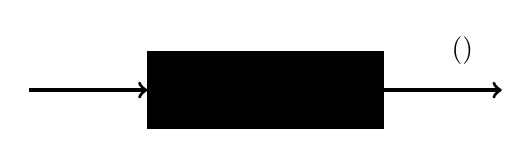
\begin{tikzpicture}[scale=1]
\fill [black] (0,0) rectangle (3,1);
\draw [->, very thick] (-1.5,0.5) -- (0,0.5); 
\draw [->, very thick] (3,0.5) -- (4.5,0.5);
\draw (-1,1) node {$\individual$};
\draw (4,1) node {$\fitnessFunction \left( \individual \right)$};
\end{tikzpicture}
\end{figure}
The optimization algorithms may, due to the lacking information about the
problem only act on a trial-and-error basis. As the goal of this
thesis is to compare how the Cross entropy Method and CMA compares, 
it's important to determine the metric for cost in terms of 
how many resources the algorithms consume versus performance.
Typically, and also in our case, the cost is measured in terms 
of function evaluations. The algorithms performance is considered 
in terms of search cost and solution value. Hence, the algorithm 
competes both on the quality of their solutions and how few times
they need to query the \textit{objective function}.


\subsubsection{Optimizing Tetris}


To understand how the optimization algorithms will handle 
the optimization of the policies, it's important to
know how the policy is defined. In the MDPTetris platform,
the policy is a \textit{one piece controller}. This means that the controller
is aware of the current board and the current piece, and it will place
the current piece only based on this information. As mentioned 
in section \ref{MDP}, the controller is only aware of a reduced 
feature set $\featureset = \{\feature_0,\dots,\feature_\dimensions\}$.
These features map a game state $\gameState$ to a real value:
$\feature : \MDPStates \rightarrow \mathbb{R}$. The value of the 
feature represents how significant the feature appears in the current
state. As an example, consider the a simplified feature set 
$\{\feature_0,\feature_1,\feature_2\}$ were the features are defined 
as in the following table.

\begin{center}
\begin{tabular}{l L{10cm}}
\textbf{Feature} & \textbf{Description}\\
\hline
$\feature_0$ & 
The depth of the deepest 
well on the board, where a well
is defined as a straight vertical 
line of unoccupied cells with 
occupied cell on both sides.\\
\hline
$\feature_1$ & 
Number of holes in the board. Precisely, empty cells
with all adjacent cells occupied.\\
\hline
$\feature_2$ & Height of the highest occupied cell.\\
\hline
\end{tabular}
\end{center}

Figure \ref{fig:exampleBoard} shows a Tetris board in a very reduced size
to illustrate how these feature functions perceive the board.
The well is shown as a dashed line, and the holes in the board 
are marked with $\times$.


\begin{figure}[H]
\begin{center}
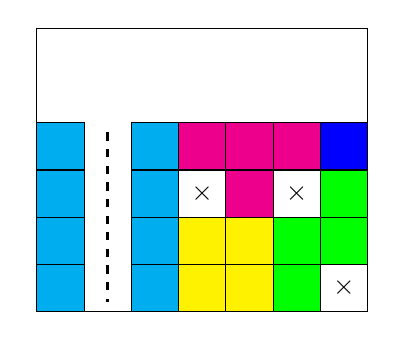
\begin{tikzpicture}[scale=0.6]
\draw  (0,0) rectangle (7,6);
\draw [fill, cyan] (0,4) node (v1) {} rectangle (1,0);
\draw  (v1) rectangle (1,3);
\draw  (0,3) rectangle (1,2);
\draw  (0,2) rectangle (1,1);
\draw  (0,1) rectangle (1,0);
\draw  [fill, cyan] (2,4) node (v2) {} rectangle (3,0);
\draw  (v2) rectangle (3,3) node (v11) {};
\draw  (2,3) rectangle (3,2);
\draw  (2,2) rectangle (3,1) node (v4) {};
\draw  (2,1) rectangle (3,0);
\draw [fill, yellow]  (5,0) rectangle (3,2) node (v3) {};
\draw  (v3) rectangle (4,1) node (v5) {};
\draw  (4,2) rectangle (5,1) node (v7) {};
\draw  (v4) rectangle (4,0);
\draw  (v5) rectangle (5,0);
\draw  [fill,green](5,2) node (v6) {} rectangle (6,0);
\draw  [fill,green](6,3) node (v8) {} rectangle (7,1);
\draw  (v6) rectangle (6,1);
\draw  (v7) rectangle (6,0);
\draw  (v8) rectangle (7,2);
\draw  (6,2) rectangle (7,1);
\draw [fill, magenta] (3,4) node (v9) {} rectangle (6,3);
\draw [fill, magenta] (4,3) rectangle (5,2);
\draw  (4,3) rectangle (5,2);
\draw  (v9) rectangle (4,3) node (v10) {};
\draw  (4,4) rectangle (5,3);
\draw  (5,4) rectangle (6,3);
\draw  (v10) rectangle (5,3);
\node (h1) at (1.5,4) {};
\node (h2) at (1.5,0) {};
\draw [very thick, dashed] (h1) -- (h2);
\draw (3.5,2.5) node {$\times$};
\draw (5.5,2.5) node {$\times$};
\draw (6.5,0.5) node {$\times$};
\draw [fill, blue]  (6,4) rectangle (7,3);
\draw (6,4) rectangle (7,3);
\end{tikzpicture}
\end{center}
\caption{Reduced example board \label{fig:exampleBoard}}
\end{figure}

When the controller is about to make a choice, it will
consider all possible locations to drop the piece. Each
of the locations corresponds to an action in the MDP.
To decide which action to take, a value function $\valueFunction$
is used to assert the value of the state. Note that 
this value function nit \textbf{not} the same as the value 
function described in section \ref{MDP}. This value function
maps a feature set and a set of associated weights to a real value.
The value from this function is used to \textit{rank} each possible action.
this function is formally defined as
\begin{align*}
\valueFunction (\gameState ) &= 
\sum_{i=1}^{\dimensions} \weight _{i}\feature _{i}(\gameState )
\end{align*}
With this function, the $i$'th weight determines how
much the $i$'th feature contribute to the decision making.
In the case with figure \ref{fig:exampleBoard}, the features yield
the following values
\begin{align*}
\feature_0 \left( \gameState \right) = 4\\
\feature_1 \left( \gameState \right) = 3\\
\feature_2 \left( \gameState \right) = 4
\end{align*}
If all weight were set to $-1$, then the controllers perception 
of the state would be
\begin{align*}
\valueFunction (\gameState ) &= 
\weight_0 \feature_0 \left( \gameState \right) + 
\weight_1 \feature_1 \left( \gameState \right) + 
\weight_2 \feature_2 \left( \gameState \right)\\
&= -4 -3 -4\\
&= -13
\end{align*}
When the controller simulates all possible actions, it will
use the very same function on the state that each action transition 
to and rank them in non-descending order. Thus, if the controller
have the actions $\{\MDPAction_0,\dots,\MDPAction_n\}$ and action 
$\MDPAction_i$ transitions to state $\gameState_i$, the controller will
order all the actions such that
\begin{align*}
\valueFunction \left( \gameState_0 \right) \geq \dots \geq 
\valueFunction \left( \gameState_n \right)
\end{align*} 
And then choose action $\MDPAction_0$. The policy of the agent 
is then defined by the combination of feature set and the set of weights.\\
\\
When applying an optimization algorithm to Tetris, the feature set is 
fixed, and the task of the optimizer is to tune the weights to make the 
policy as efficient as possible. This is done through the previously 
mentioned \textit{Monte Carlo} method, where the agent is simulated
with a given policy from the starting state, and the final score is 
used to determine the performance of the policy. The next sections 
walks through how the optimizers each approach this task.

\maybe{
The \textit{black box} search can be applied very well
in the search of policies for Tetris. As described in
section \ref{MDP}, to learn the performance of a policy from
a state $\MDPValueFunction^{\policy} \left( \MDPState \right)$,
the agents is simulated with the policy in the state, and once the
simulation ends, the final value from the function is how much reward
the agent accumulated during the game from the given state,
where the reward is the number of lines cleared during the game.\\




The optimizing algorithms used in this thesis both attempts to 
optimize a certain function. In this case, the optimization 
function aims to develop the best possible Tetris playing agent.
Thus, the value of the objective function describes an estimated 
performance of the input agent. The objective function serves as
an abstraction to the Tetris emulator that will evaluate 
the agent by letting the agent play a pre-configured number 
of games. The objective function that estimates the performance 
of an agent is later referred to as $\fitnessFunction$.\\
\\
When the Tetris simulator plays Tetris, the internal decision process
of the Tetris controller is configured with a set of parameters which remain
fixed across a single game. These parameters are the weights associated 
with each feature function that is considered by the controller. 
The features $\feature _{i}$
each map a state $\gameState$ of the game to a real value. 
An overview of the exact mappings
can be seen in table 1 in \citep{scherrer2009:b}. How much each of these mappings
should affect the final evaluation of the board is determined by $\weight _{i}$
denoting the weight of the $i$-th feature.
Finally, the function to assess the value 
of current board state $\valueFunction \left( \gameState \right)$, 
with $\dimensions$ features functions present, can be expressed as:
\begin{align*}
\valueFunction (\gameState ) &= 
\sum_{i=1}^{\dimensions} \weight _{i}\feature _{i}(\gameState )
\end{align*}
Let $\allGameStates$ be the set of all states that each possible 
action can lead to from the current state $\gameState$. The 
controller will then for each reachable state 
$\gameState_i \in \allGameStates$ evaluate the state by 
$\fitnessFunction \left( \gameState_i \right)$. 
The chosen action is the one that yields the state of the highest value.
The performance of the controller is hence directly tied to the 
features and weights in the evaluation function. To adjust these controllers,
one can either change the set of applied feature functions, or as the 
optimization algorithms will do, change the weighting of the features.
For the experiments, the feature sets remain fixed, and the task of the
optimization algorithm applied is to tune the set of weights in order 
to maximize the performance of the controller.\\
\\
In summary, the objective function accepts a vector of values for each weight
and configures an agent with the weights corresponding to the entries in
the input vector. It then plays $\numberOfEvaluations$ games with the
agent and reports the mean score.
}
\tmpcom{
% evaluating a specific agent
Now that the new generation has been created, 
it's time for each agent to play g games of Tetris.\\
For a given Tetris game, we say that a game consists 
of a range of states. A state is defined as, when an 
agent has to place a given piece, and it has to choose 
where to place the piece on the board. Placing the 
piece is called an action, and since there are multiple 
ways to place the piece on the board, we have a range 
of possible of actions. In a given state the agent 
has to try each possible action, and the action 
with the highest evaluation, is the action the 
agent executes in the current state. 
When evaluating each possible action, the 
objective function S is used. As shown in the 
input-section, the objective function is 
defined as:
\begin{align*}
\valueFunction (\gameState ) &= \sum_{i=1}^{\dimensions} \weight _{i}\feature _{i}(\gameState )
\end{align*}

Where $F_i$ is the i'th feature function 
and w\_i is the i'th weight associated 
with the corresponding i'th feature function. 
More specifically w\_i is the value of 
the i'th dimension of the agent's vector.
A specific action then gets evaluated 
by computing S(x). The main factor of 
the evaluation value is how the action 
changed the board layout , since each 
feature function F\_i (x) looks at different 
"types" of board layouts (insert ref. to feature policy table).
}


